\section*{Summary}
A great summary of ridge regression and lasso, as well as some implementation tips, can be found on the website given in \cite{Kas2018}. A Notebook going through Lab 2 of ISLR can be found in the website given in the footnote\footnote{http://www.science.smith.edu/~jcrouser/SDS293/labs/lab10-r.html}\\
\\
In this chapter we summarize for our-self what we are eventually going to write about in the paper.

\subsection*{The Elements of Statistical Learning}
All of the information below came from the book "Elements of Statistical Learning", unless stated otherwise.

\subsubsection*{Introduction}
Learning problems
\begin{itemize}
    \item Supervised learning: predict the value of an outcome measure based on a number of input measures (f.e. regression).
    \item Unsupervised learning: No outcome measure, goal is to describe the associations and patterns in input measures (f.e. classification).
\end{itemize}

\subsubsection*{Chapter 3: Linear methods for regression}
Linear regression
\begin{itemize}
    \item Given is a data matrix containing $N$ data vectors $x_i \in \mathbb{R}^p$ \begin{equation*}
        \textbf{X} = \begin{pmatrix}
        1 & x_{11} & x_{12} & \dots & x_{1p}\\
        1 & x_{21} & x_{22} & \dots & x_{2p}\\
        \vdots & \vdots & \vdots & \ddots & \vdots\\
        1 & x_{N1} & x_{N2} & \dots & x_{Np}
        \end{pmatrix}
    \end{equation*}
    where we assume that its column space has full rank.
    \item We want to minimize the Residual Sum of Squares: \begin{equation*}
        \text{RSS}(\beta) = (\textbf{y} - \textbf{X}\beta)^T(\textbf{y} - \textbf{X}\beta).
    \end{equation*}
    \item This is achieved for $\beta = (\textbf{X}^T\textbf{X})^{-1}\textbf{X}^T\textbf{y}$.
    \item We denote the predicted values as $\hat{y}$ and calculate them as \begin{equation*}
        \hat{y} = \textbf{X}\beta = \textbf{X}(\textbf{X}^T\textbf{X})^{-1}\textbf{X}^T\textbf{y} = \textbf{H}y.
    \end{equation*}
    The matrix $\textbf{H}$ is often called the \textit{hat} matrix as it \textit{puts the hat on the vector \textbf{y}}. It projects the vector $\textbf{y}$ orthogonally onto the column space of \textbf{X}.
    \item Gauss-Markov theorem: The least squares estimator of $\beta$ is the one with the smallest variance among all linear unbiased estimators of $\beta$. There could, however, exist biased estimators with smaller mean squared error (= variance).
\end{itemize}
An example of linear regression (on prostate cancer) starts on p. 49. This example will return later in the section about the $LASSO$-estimator.\\
\\
Chapter 3.2.3: "Multiple regression from simple univariate regression" is pretty vague, I don't understand it. \\
\\
Problems with least squares estimates:
\begin{itemize}
    \item Prediction accuracy: Least squares estimates have low bias but large variance. Sacrificing a little bit of bias to reduce variance might improve the overall accuracy.
    \item Least squares estimates take all variables into account. For the sake of easy to interpret models, it is sometimes advisable to reduce the number of variables (and therefor sacrificing some bias) to better understand "the big picture" (i.e. see what variables matter the most when trying to predict certain outcomes).
\end{itemize}
This brings us to subset selection.
\begin{itemize}
    \item Subset selection looks to retain only a subset of the variables and eliminate the rest from the model.
    \item \textit{Best-subset selection}: Finds for each $k$ the subset of size $k$ that gives the smallest residual sum of squares. The higher $k$, the lower $RSS$, but the more complex the model becomes.
    \item \textit{Forward-stepwise selection}: Starts with the intercept and sequentially adds predictors that most improve the fit.
    \item \textit{Backward-stepwise selection}: Starts with the full model and sequentially deletes predictors that have the least impact on the fit.
    \item \textit{Forward-stagewise regression}: (probably) not important for our topic.
\end{itemize}
\underline{\textbf{3.4:} Shrinkage methods}\\
Often times subset selection is too 'crude' of a method to reduce the prediction error of the full model as it is a discrete method: It either retains or discards a predictor. Shrinkage methods are more continuous and don't suffer as much from high variability. 

\begin{itemize}

    % The ridge estimator
    \item \textit{Ridge regression}: Ridge regression shrinks the regression coefficients by imposing a penalty on their size. Unlike normal linear regression, where one tries to minimize the Residual Sum of Squares \begin{equation*}
        \text{RSS}(\beta) = \argmin_{\beta}\bigg\{\sum_{i=1}^N \bigg( y_i - \beta_0 - \sum_{j=1}^p x_{ij}\beta_j\bigg)^2\bigg\}
    \end{equation*}
    we minimize the following expression \begin{equation}\label{eq:ridgeEstimator}
        \hat{\beta}{}^{\text{ridge}} = \argmin_{\beta}\bigg\{\sum_{i=1}^N \bigg( y_i - \beta_0 - \sum_{j=1}^p x_{ij}\beta_j\bigg)^2 + \lambda \sum_{i=1}^p \beta_i^2\bigg\}
    \end{equation}
    where $\lambda$ is the complexity parameter, it controls how much the coefficients are shrunk. Equivalently, we can write equation \eqref{eq:ridgeEstimator} as \begin{equation}\label{eq:ridgeEstimatorEquivalent}
    \begin{aligned}
        \hat{\beta}{}^{\text{ridge}} = \argmin_{\beta}\bigg\{\sum_{i=1}^N \bigg(y_i - \beta_0 - \sum_{j=1}^p x_{ij}\beta_j\bigg)^2\bigg\} \newline \text{, subject to } \sum_{i=1}^p \beta_i^2 < t
    \end{aligned}
    \end{equation}
    which explicitly states the size constraint on the parameters. Ridge regression is to be preferred over normal regression when there are many correlated variables in the model, as that can lead to variables getting very large positive and negative coefficients that ultimately cancel each other out (say for example $y = 10^{16}x_1 - 5*10^{15}x_2$). By imposing a size constraint on the parameters, this problem is alleviated.\\
    \\
    \textbf{(For question 2)} Also notice that the intercept coefficient $\beta_0$ has been left out of the penalization. Penalization of the intercept would make the procedure depend on the origin chosen for $Y$, that is, say we shift $Y$ in some direction by adding a constant $c$ to its components, then this would not simply result in a shift of the predictions by the same amount $c$.\\
    \\
    Writing equation \eqref{eq:ridgeEstimator} in matrix notation (after centralizing the data and setting $\beta_0 = \frac{1}{N} \sum_{i=1}^N y_i$) with $\beta = (\beta_1, \dots \beta_p)$, we get
    \begin{equation}\label{RidgeMatrixNotation}
        RSS(\lambda) = (\textbf{y} - \textbf{X}\beta)^T(\textbf{y} - \textbf{X}\beta) + \lambda\beta^T\beta
    \end{equation}
    The solution to this minimization problem can be seen to be
    \begin{equation}
        \hat{\beta}{}^{\textrm{ridge}} = (\textbf{X}^T\textbf{X} + \lambda\textbf{I})^{-1}\textbf{X}^T\textbf{y}.
    \end{equation}
    We define the \textit{effective degrees of freedom} of the ridge regression fit to be \begin{align*}
        \textrm{df}(\lambda) & = \textrm{tr}[\textbf{X}(\textbf{X}^T\textbf{X} + \lambda\textbf{I})^{-1}\textbf{X}^T]\\
        & = \sum_{i=1}^p \frac{d_j^2}{d_j^2 + \lambda}
    \end{align*}
    The coefficients $d_j$ come from the singular value decomposition (SVD) of the data-matrix \textbf{X} \begin{equation*}
        \textbf{X} = \textbf{UDV}^T.
    \end{equation*}
    Here $\textbf{U} \in \mathbb{R}^{N \times p}$, $\textbf{D} \in \mathbb{R}^{p \times p}$ and $\textbf{V} \in \mathbb{R}^{p \times p}$. The matrices \textbf{U} and \textbf{V} are orthonormal matrices and the matrix \textbf{D} is a diagonal matrix containing the singular values $d_j$ with $d_1 \geqslant d_2 \geqslant \dots \geqslant d_p$ of \textbf{X}.\\
    \\
    Substituting \textbf{X} with its SVD in the formula for the regular regression coefficients, we obtain
    \begin{align*}
        \textbf{X}\beta &  = \textbf{X}(\textbf{X}^T\textbf{X})^{-1}\textbf{X}^T\textbf{y}\\
        & = \textbf{U}\textbf{U}^T\textbf{y}.
    \end{align*}
    It can be shown that $\textbf{U}\textbf{U}^T = \textbf{H}$ is the orthogonal projector onto the column space of \textbf{X}. Doing the same for the ridge estimator $\hat{\beta}{}^{\textrm{ridge}}$ we obtain
    \begin{align*}
        \textbf{X}\hat{\beta}{}^{\textrm{ridge}} & = \textbf{X}(\textbf{X}^T\textbf{X} + \lambda\textbf{I})^{-1}\textbf{X}^T\textbf{y}\\
        & = \sum_{j=1}^p \textbf{u}_j\frac{d_j^2}{d_j^2 + \lambda}\textbf{u}_j^T\textbf{y}
    \end{align*}
    We see that, like linear regression, ridge regression computes the coordinated of \textbf{y} with respect to the orthonormal basis \textbf{U}. It then shrinks these coordinates with the factor $\frac{d_j^2}{d_j^2 + \lambda}$. This means that a greater amount of shrinkage is applied to the coordinates of basis vectors that correspond to smaller $d_j$'s. It can be shown that the values $d_j$ also correspond to the principal components of \textbf{X} (see book p. 66). The smallest principle component $d_p$ is the one that explains the least amount of variance of the model and gets shrunk the most.
    
    % The lasso estimator
    \item \textit{The Lasso}: Very similar to ridge regression, the lasso\footnote{Least Absolute Shrinkage and Selection Operator, \cite{Kas2018}} is also a shrinkage method but there is a subtle yet important difference. The lasso estimate is defined by \begin{equation}\label{eq:lassoEstimate}
        \hat{\beta}{}^{\textrm{lasso}} = \argmin_{\beta}\bigg\{\frac{1}{2}\sum_{i=1}^N \bigg(y_i - \beta_0 - \sum_{j=1}^p x_{ij}\beta_j\bigg)^2 + \lambda \sum_{i=1}^p |\beta_i|\bigg\}
    \end{equation}
    or equivalently,
    \begin{equation*}
        \begin{aligned}
        \hat{\beta}{}^{\text{lasso}} = \argmin_{\beta}\bigg\{\sum_{i=1}^N \bigg(y_i - \beta_0 - \sum_{j=1}^p x_{ij}\beta_j\bigg)^2\bigg\} \newline \text{, subject to } \sum_{i=1}^p |\beta_i| < t.
    \end{aligned}
    \end{equation*}
    As can be seen from the definitions, the ridge and lasso estimates only differ in how they measure the size of the regression coefficients $\beta$. The ridge estimate measures $\beta$ in $L_2$ norm (also known as Euclidean distance) while the lasso estimate measures $\beta$ in $L_1$ norm (which is also known as Manhattan or Taxicab distance)\footnote{The existence of the ridge and lasso estimate could imply the existence of a whole class of estimates similar to ridge and lasso, but differing in what norm $L_p$ they use to measure the size of $\beta$. This is indeed the case: this class of estimators is known as the Bridge estimators \cite{WWM2020}. It is even possible to let $p$ take on non-integer values. If we set $p=0$, the method corresponds to variable subset selection as the penalty simply counts the number of non-zero parameters.}.
\end{itemize}

\underline{\textbf{3.4.3:} A comparison between subset selection, ridge estimates and lasso estimates.}
\begin{itemize}
    \item subset-selection: hard thresholding $\rightarrow$ A predictor is either included or excluded.
    \item ridge and lasso estimates: soft thresholding $\rightarrow$ Shrinkage of coefficients.
\end{itemize}
Both the ridge and lasso methods can be visualized by figure~\ref{fig:Fig3.11}.
\begin{figure}[h!]
    \centering
    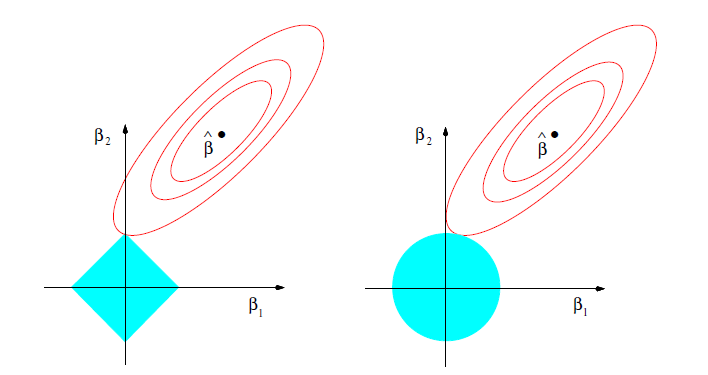
\includegraphics[width=\linewidth]{Figures/Figure3.11.PNG}
    \caption{Figure 3.11 from the book}
    \label{fig:Fig3.11}
\end{figure}
The methods find the first intersection of the region $L_p(\beta) < t$ and the elliptical contours of the residual sum of squares. The region $L_p(\beta) < t$ is a circle of if $p=2$ and diamond-shaped if $p=1$. Ideally, we would like the intersection to be at a point where (many) $\beta_j$'s are zero, so we can simplify the model. Different elements of the bridge estimator class give rise to different blue regions.\\
\\
\underline{Eigen hersenspinsel, niet te veel aandacht aan besteden.}\\
A possibly interesting case is $p=0$, then the region is defined as $\{(x,y) \hspace{3pt} | \hspace{3pt} x^0 + y^0 = t\}$. The only possible value $t$ can take in this case is $1$ or $2$, corresponding to the the $x$-and $y$-axis, respectively the whole plain where we defined $0^0=0$.\\
\\
As a side note, the lasso, ridge regression and best subset selection can all be viewed as Bayes estimators of the correct prior distributions. Lastly, it is also possible to combine estimators. An example of this is the estimator introduced by Zou and Hastie (2005), which uses the \textit{Elastic-net} penalty \begin{equation*}
    \lambda\sum_{j=1}^p (\alpha\beta_j^2+(1-\alpha)|\beta_j|).
\end{equation*} It combines aspects from both ridge and lasso estimates and can be advantages in certain situations (especially computationally).\\
\\
\underline{\textbf{3.4.4:} Least Angle Regression (LAR)}
\begin{enumerate}
    \item Identify the predictor $x_i$ that is most correlated with the response.
    \item Move the coefficient $\beta_i^{\textrm{LAR}}$ of this predictor continuously towards its least squares coefficient $\beta_i^{\textrm{ls}}$, causing its correlation with the residual to decrease. In other words: try to find the variable that explains the most variance of the complete model en include it more and more into the new model.
    \item As soon as an other predictor $x_j$ "catches up" in terms of correlation with the residual, $x_j$ joins the active set and their coefficients are moved together towards their full least squares coefficients in such a way that the correlation of $x_i$ and $x_j$ with the response stays equal. This process ends at the full least squares fit.
\end{enumerate}
See also Algorithm 3.2 in the book on page 74.\\
\\
It can be shown that by a simple modification of this algorithm, an algorithm for the lasso estimate can be achieved (Algorithm 3.2a, page 76).\\
\\
Section 3.8 expands further on Lasso.

% ------------------------------------------------------------
% ----- Introduction to Statistical Learning: Chapter 5 ------
% ------------------------------------------------------------

\subsection*{Introduction to Statistical Learning (Chapter 5: Resampling methods)}
The aim of this section is to compile some important elements surrounding (cross-)validation. All of the information below came from the book "Introduction to Statistical Learning", unless stated otherwise.

\underline{Introduction}
\begin{itemize}
    \item Cross-validation can be used to estimate the test error associated with a given statistical learning method in order to evaluate its performance (also known as \textit{Model assessment}.
    \item Cross-validation can also be used to select the appropriate level of flexibility (also known as \textit{Model selection}.
\end{itemize}

\underline{Cross-validation}
\begin{itemize}
    \item Problem: How to test whether a statistical model is a good model? Solutions: \begin{itemize}
        \item Use a test set (a set of data that is not used in the deriving of the model) to check whether the predictions match the data.\\
        \textbf{Problem:} Such a set is often not available.
        \item Use training data to check whether the predictions match the data. \\
        \textbf{Problem:} Such a test often grossly underestimates the true \textit{test error}.
        \item Make some perturbations on the training data and calculate the expected result. Then check whether the model predicts this expected result.
        \item Hold out a subset of the training data and test the derived model with this subset. It is this type of testing we're interested in.
    \end{itemize}
\end{itemize}

\underline{Validation set approach}
\begin{itemize}
    \item Randomly divide the observations into a \textit{training set} and a \textit{test set}. Derive a model based on the training set data.
    \item The validation set test error provides an estimate for the test error of the model (often measured in MSE).
    \item Problems: \begin{itemize}
        \item Since not all available data is used in the models (some of it is used to test the model), it can be expected that the estimated test error is higher than the test error that one would get when deriving the model based on all available data.
        \item Since we randomly divide the observations into two sets, there is a variability in the estimated test error. This variability tends to be quite high.
    \end{itemize}
\end{itemize}

\underline{Leave-On-Out Cross-validation (LOOCV)}
\begin{itemize}
    \item Apply the \textit{Validation set approach} as described above with a test set containing precisely one observation and the training set the other $n-1$ observations. Derive the model with the training set data and calculate the test error of the single test set element, call it $MSE_1$. Repeat this procedure $n$ times, one time for each element $y_i$ in the training set, with $\{y_i\}$ the test set. An estimation for the test error is then \begin{equation*}
        CV_{(n)} = \frac{1}{n}\sum_{i=1}^n MSE_i.
    \end{equation*}
    \item Tends to be computationally expensive as $n$ gets large.
    \item A nice shortcut exists in the case of least squares linear or polynomial regression. see page $180$.
\end{itemize}

\underline{K-fold Cross-Validation}
\begin{itemize}
    \item The observations are split into $k$ subsets of approximately equal size (also called \textit{folds}). The first fold is treated as the validation set, the other $k-1$ folds are used together as the training set. We then calculate the test error $MSE_1$ with the validation set. This process is repeated $k$ times, where each time we use a different fold as the validation set. An estimate for the test error is then \begin{equation*}
        CV_(k) = \frac{1}{k}\sum_{i=1}^k MSE_i
    \end{equation*}
    \item It is clear that LOOCV is a special case of $K$-fold CV. General $K$-fold CV has obvious computational advantages over LOOCV.
    \item In general, $5$- or $10$-fold Cross-validation is a more accurate test error estimation method than LOOCV. This might be surprising at first: Since we use more of the available data in LOOCV, we should expect LOOCV the be more accurate. While it is true that the bias of LOOCV is lower than, say, $10$-fold Cross-validation (for the model tested in LOOCV is nearly the model when using all available data, unlike the model tested in $10$-fold Cross-validation), it does not tell the whole story, variance must also be taken into account. Since the training data in LOOCV for each model is nearly identical, the test error estimates are going to be very correlated, leading to a high test error variance\footnote{A small change in one test error will imply nearly the same change in all other test errors because they are very correlated. Thus, the average of all test errors will have high variability.}. In the case of $10$-fold Cross-validation, this correlation will be much less, leading to a lower test error variance. The slight increase in bias is thus well made up for by the big decrease in variance, to such an extend that $10$-fold Cross-validation is better than LOOCV. (\textit{bias-variance trade-off})
\end{itemize}

% ------------------------------------------------------------
% ----- Introduction to Statistical Learning: Chapter 6 ------
% ------------------------------------------------------------

\subsection*{Introduction to Statistical Learning (Chapter 6: Linear model selection and Regularization)}
All of the information below came from the book "Introduction to Statistical Learning", unless stated otherwise.

\subsubsection*{Important notions}
In this subsection we list some important notions to understand what is written below.
\begin{itemize}
    \item Training error: The error (measured in RSS, $R^2$, \dots) of the training data with respect to the predicted values.
    \item Test error: The error (measured in RSS, $R^2$, \dots) of the test data with respect to their predicted values. Notice the important difference with training error: the parameters of the model were chosen based to best fit the training data, hence the training error will be as low as possible. The data from the test error, however, has had no influence on the model and is thus a better measure of 'how good' the model is.
    \item Null model: a model that contains no predictors.
    \item Cross-validation: Use test data to asses how good the model is (measure what the prediction error is). See also previous chapter.
    \item We say that \textit{a model has high variance} if a small change in training data leads to substantial changes in the coefficients $\beta$.
    \item Sparse model: models that involve only a subset of the variables.
\end{itemize}

\subsubsection*{Introduction}
Why do we want alternative procedures for least squares fitting?
\begin{itemize}
    \item \textit{Prediction accuracy}: If $n >> p$, then least squares fitting will have low variance. However, if $n$ is not much larger than $p$, least squares fitting tends to have high variance (overfitting). If $p > n$, then the variance is even infinite. By constraining or shrinking the estimated coefficients, we can lower the variance substantially at the cost of a minor increase in bias.
    \item \textit{Model interpretability}: Removing unnecessary variables improves the interpretablility of the result.
\end{itemize}

\subsubsection*{Subset selection}
\underline{Best subset selection}
\begin{itemize}
    \item Consider all subsets of $k$ predictors from the full model (with $n$ predictors). Calculate for each the least squares regression fit and pick the one with the lowest \textit{test error}.
    \item This method is computationally heavy and becomes unfeasible if $n > 40$.
\end{itemize}

\underline{Forward stepwise selection}
\begin{itemize}
    \item Algorithm: 
        \begin{enumerate}
        \item Start from the null model $\mathcal{M}_0$.
        \item Add the predictor that augments the current model the most. That is, find the predictor $x_{k+1}$ such that $\mathcal{M}_{k} \cup x_{k+1}$ has the lowest RSS. In this way, one achieves a sequence of models $\mathcal{M}_0, \mathcal{M}_1, \dots, \mathcal{M}_p$.
        \item Use cross-validation to select the best model in the above sequence. 
        \end{enumerate}
    \item This method is not guaranteed to find the best subset. 
\end{itemize}

\underline{Backwards stepwise selection}
\begin{itemize}
    \item Same as Forward stepwise selection, but instead of starting with a null model and sequentially adding predictors, we start with the full model and sequentially remove predictors.
    \item This method is not guaranteed to find the best subset.
\end{itemize}

\underline{Hybrid models}
Like Forward stepwise selection, but now at each step it is checked if a variable in the model is no longer useful so that it can be removed. This method tries to mimic better best subset selection.

\underline{Choosing the optimal model: What statistic to use?}
Section 6.1.3 in the book (p. 210). Could be useful.

\subsubsection*{Shrinkage methods}
Instead of using subsets, we use all $p$ predictors but restrain the coefficient estimates. This significantly reduces the variance of the model.\\
\\
\underline{Ridge regression}
\begin{itemize}
    \item Instead of minimizing the Residual Sum of Squared \begin{equation*}
        RSS = \sum_{i=1}^n \bigg( y_i - \beta_0 - \sum_{j=1}^p x_{ij}\beta_j\bigg)^2,
    \end{equation*} we minimize
    \begin{equation*}
        \sum_{i=0}^n \bigg( y_i - \beta_0 - \sum_{j=1}^p x_{ij}\beta_j\bigg)^2 + \lambda \sum_{i=1}^p \beta_i^2 = RSS + \lambda \sum_{i=1}^p \beta_i^2
    \end{equation*}
    where $\lambda$ is called the tuning parameter and $\sum_{i=1}^p \beta_i^2$ is called the \textit{shrinking penalty}. Note that we do not penalize the intercept coefficient $\beta_0$. After centering of the data, that is, the column of $\textbf{X}$ have been centered to have mean zero, $\beta_0$ can be calculated as $\beta_0 = \frac{1}{n}\sum_{j=1}^n y_j$.
    \item As $\lambda$ increases, the coefficients do not necessarily decrease! It is however most of the time the case that coefficients decrease as lambda increases.
    \item It is very much advisable to standardise the data before applying ridge regression, as it is very sensitive to scale changes.
    \item Ridge regression is best used in cases were normal regression has high variance (f.e. if $n$ is close to $p$ or even smaller than $p$).
    \item Computationally, ridge regression is almost as fast as normal least squares fitting.
\end{itemize}

\underline{The Lasso}
\begin{itemize}
    \item Motivation: Ridge regression always keeps all predictors (it merely shrinks their coefficients). From a perspective of model interpretation, this is not desirable. Lasso estimation looks to solve this shortcoming.
    \item The lasso estimate minimizes
    \begin{equation*}
        \sum_{i=1}^n \bigg( y_i - \beta_0 - \sum_{j=1}^p x_{ij}\beta_j\bigg)^2 + \lambda \sum_{i=1}^p |\beta_i| = RSS + \lambda \sum_{i=1}^p |\beta_i|.
    \end{equation*}
    Notice that the only difference with the ridge estimation is the norm in which we measure $\beta$. Also notice the slight change in definition of this estimator between the two books.
    \item If the tuning parameter $\lambda$ is sufficiently large, it will have the effect that some coefficients will be exactly zero. Hence, lasso performs variable selection (much like subset selection methods). We say that lasso (and subset selection methods) generate spare models.
    \item The most suitable value for $\lambda$ is to be chosen based on cross-validation.
    \item Lasso implicitly assumes some of the true coefficients of $\beta$ are zero.
     \item Lasso performs what is known as \textit{soft thresholding}: It sets coefficients to zero as soon as a certain threshold is reached, above that threshold, coefficients vary continuously.
\end{itemize}

\underline{Alternative formulation for ridge regression and the Lasso}
\begin{itemize}
    \item Very similar as was explained in the previous book, although it's explained nicer here. See pages 220-221.
\end{itemize}

\underline{The variable selection property of Lasso}
\begin{itemize}
    \item Nice pictorial explanation (p. 221-223).
\end{itemize}

\underline{Comparing the Lasso and ridge regression}
\begin{itemize}
    \item If non of the true coefficients of $\beta$ equal zero, ridge estimates outperform lasso estimates in terms of prediction error. The roles are reversed is some of the true coefficients of $\beta$ are in fact equal to zero.
    \item See also the section about the special case for more intuition (page 224-225).
\end{itemize}

\underline{Selecting the tuning parameter}
\begin{itemize}
    \item To Do: Read about cross-validation first as it appears to be important in this section.
\end{itemize}